\subsection{QuizziPedia::Back-End::App::Routers}
\subsubsection{Informazioni generali}
\label{QuizziPedia::Back-End::App::Routers}
\begin{figure}[ht]
	\centering
	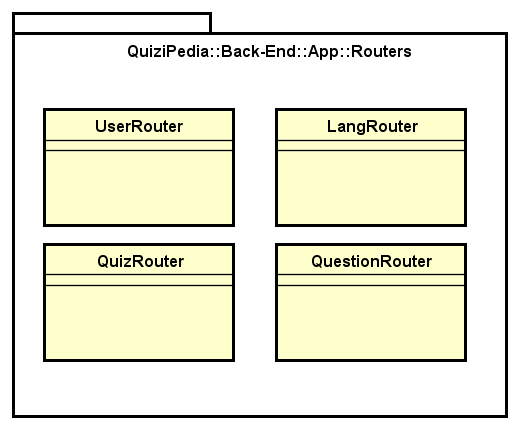
\includegraphics[scale=0.7]{UML/Package/QuizziPedia_Back-End_App_Routers.png}
	\caption{QuizziPedia::Back-End::App::Routers}
\end{figure}
\FloatBarrier
	\begin{itemize}
		\item \textbf{Descrizione}: 
		\textit{package\ped{G}} contenente i router della componente back-end dell'applicazione. Contiene i file di configurazione relativi al routing delle richieste del \textit{client\ped{G}}, ossia i \textit{routers} di \textit{Express\ped{G}};
		\item \textbf{Padre}: \texttt{App};
		\item \textbf{Interazioni con altri componenti}:
			\begin{itemize}
				\item \texttt{Controllers}: \textit{package\ped{G}} che contiene i \textit{Controllers} di \textit{Express\ped{G}}, definisce la logica dell'applicazione.
			\end{itemize}
	\end{itemize}
\subsubsection{Classi}

\paragraph{QuizziPedia::Back-End::App::Routers::UserRouter}
\label{QuizziPedia::Back-End::App::Routers::UserRouter}
\begin{figure}[ht]
	\centering
	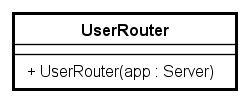
\includegraphics[scale=0.45]{UML/Classi/Back-End/QuizziPedia_Back-End_App_Routers_UserRouter.png}
	\caption{QuizziPedia::Back-End::App::Routers::UserRouter}
\end{figure}
\FloatBarrier
	\begin{itemize}
		\item \textbf{Descrizione} \\
		Classe che gestisce le richieste relative alla registrazione, alla gestione della sessione e alla cronologia dei questionari svolti di un utente.
Componente ConcreteHandler del design pattern \textit{Chain of responsibility\ped{G}}. Utilizza il modulo \textit{Passport\ped{G}}.
		\item \textbf{Utilizzo} \\
		Viene utilizzata per chiamare il controller che si occupa di gestire le API relative alla registrazione, alla gestione della sessione e alla cronologia dei questionari di un utente.
		\item \textbf{Relazioni con altre classi} 
		\begin{itemize}
		\item 
			IN	\texttt{Server}\\
			Classe che avvia il server. Nello specifico apre una connessione al database tramite \textit{Mongoose\ped{G}}, invoca il middleware \textit{Express\ped{G}} passando un riferimento al database MongoDB come parametro in modo che possa configurarsi con esso, invoca il \textit{middleware\ped{G}} \textit{Passport\ped{G}} ed infine si mette in ascolto su una determinata porta. È il componente client del design pattern \textit{Chain of responsibility\ped{G}}. Utilizza i moduli \textit{Mongoose\ped{G}}, \textit{Express\ped{G}}, \textit{Passport\ped{G}}. 
		\item 
			OUT \texttt{ErrorHandler}\\
			Classe \textit{middleware\ped{G}} per la gestione degli errori. Ritorna al client un oggetto di tipo Response con stato \textit{HTTP\ped{G}} 500 e descrizione dell’errore in formato \textit{JSON\ped{G}}. È un
componente ConcreteHandler del design pattern \textit{Chain of responsibility\ped{G}}.
		\item 
			OUT \texttt{NotFoundHandler}\\
			Classe che si occupa della gestione dell’errore di pagina non trovata. Componente ConcreteHandler del design pattern \textit{Chain of responsibility\ped{G}}.
		\item 
			OUT \texttt{UserController}\\
			Classe che raggruppa attraverso require i vari controllers responsabili delle operazioni legate alla gestione degli utenti. Si è scelto di predisporre questo raggruppamento per facilitare l'introduzione di nuove funzionalità legate alla gestione degli utenti.
		\item 
			OUT \texttt{SummaryController}\\
			Classe che gestisce la cronologia dei questionari svolti dall'utente
	\end{itemize}
		\item \textbf{Metodi} 
		\begin{itemize}
		\item 
		\texttt{+ UserRouter(app: Server)} \\
		Contiene diverse route che vengono configurate all’avvio del server. Quest’ultime ricevono le richieste del client e passano il controllo al ConcreteHandler successivo.
		\textbf{Parametri}:
			\begin{itemize}
				\item 
				\texttt{app: Server} \\
				Rappresenta l’istanza del server su cui configurare i route che mappano i controllers specifici.
			\end{itemize}
		\end{itemize}
\end{itemize}		
\paragraph{QuizziPedia::Back-End::App::Routers::QuestionRouter}
\begin{figure}[ht]
	\centering
	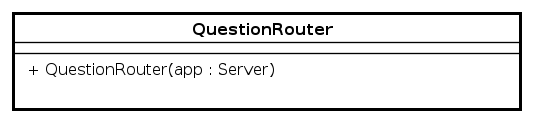
\includegraphics[scale=0.45]{UML/Package/QuizziPedia_Back-End_App_Routers_questionRouter.png}
	\caption{QuizziPedia::Back-End::App::Routers::QuestionRouter}
\end{figure}
\FloatBarrier
	\begin{itemize}
		\item \textbf{Descrizione} \\
		Classe che gestisce le richieste relative alle operazioni riguardanti le domande. Componente ConcreteHandler del design pattern Chain of responsibility.
		\item \textbf{Utilizzo} \\
		Viene utilizzata per chiamare il controller che si occupa di gestire le API relative alle domande.
		\item \textbf{Relazioni con altre classi} \\
		\begin{itemize}
			\item \textbf{IN} \texttt{Server}\\
			Classe che avvia il server. Nello specifico apre una connessione al database tramite Mongoose, invoca il middleware Express passando un riferimento al database MongoDB come parametro in modo che possa configurarsi con esso, invoca il middleware Passport ed infine si mette in ascolto su una determinata porta. È il componente client del design pattern Chain of responsibility. Utilizza i moduli Mongoose, Express e Passport.
			\item \textbf{OUT} \texttt{ErrorsHandler}\\
			Classe middleware per la gestione degli errori. Ritorna al client un oggetto di tipo Response con stato HTTP 500 e descrizione dell'errore in formato JSON. È un componente ConcreteHandler del design pattern Chain of responsibility.
			\item \textbf{OUT} \texttt{NotFoundHandler}\\
			Classe che si occupa della gestione dell’errore di pagina non trovata. Componente ConcreteHandler del design pattern Chain of responsibility.
			\item \textbf{OUT} \texttt{QuestionController}\\
			Classe che raggruppa i vari controllers responsabili delle operazioni riguardanti le domande attraverso \texttt{require}.
		\end{itemize}
		\item \textbf{Metodi} \\
		\begin{itemize}
			\item \texttt{+ QuestionRouter(app: Server)}\\
			Contiene diverse route che vengono configurate all’avvio del server. Quest’ultime ricevono le richieste del client e passano il controllo al ConcreteHandler successivo.\\
			\textbf{Parametri}:
			\begin{itemize}
				\item \texttt{app: Server}\\
				Rappresenta l’istanza del server su cui configurare i route che mappano i controllers specifici.
			\end{itemize}
		\end{itemize}
	\end{itemize}
\paragraph{QuizziPedia::Back-End::App::Routers::QuizRouter}
\label{QuizziPedia::Back-End::App::Routers::QuizRouter}
\begin{figure}[ht]
	\centering
	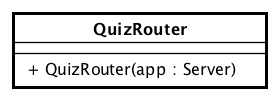
\includegraphics[scale=0.8]{UML/Classi/Back-End/QuizziPedia_Back-End_App_Routers_quizRouter.png}
	\caption{QuizziPedia::Back-End::App::Routers::QuizRouter}
\end{figure}
\FloatBarrier
	\begin{itemize}
		\item \textbf{Descrizione}: classe che gestisce le richieste relative alle operazioni riguardanti un questionario. Componente \textit{ConcreteHandler\ped{G}} del \textit{design pattern\ped{G}} \textit{Chain of responsibility\ped{G}};
		\item \textbf{Utilizzo}: viene utilizzata per chiamare il \textit{controller\ped{G}} che si occupa di gestire le \textit{API\ped{G}} relative ad un questionario;
		\item \textbf{Relazioni con altre classi}:
		\begin{itemize}
		\item \textbf{IN \texttt{Server}}: classe che avvia il \textit{server\ped{G}}. Nello specifico apre una connessione al database tramite \textit{Mongoose\ped{G}}, invoca il \textit{middleware\ped{G}} \textit{Express\ped{G}} passando un riferimento al database \textit{MongoDB\ped{G}} come parametro in modo che possa configurarsi con esso, invoca il \textit{middleware\ped{G}} \textit{Passport\ped{G}} ed infine si mette in ascolto su una determinata porta. È il componente \textit{client\ped{G}} del \textit{design pattern\ped{G}} \textit{Chain of responsibility\ped{G}}. Utilizza i moduli \textit{Mongoose\ped{G}}, \textit{Express\ped{G}}, \textit{Passport\ped{G}};
		\item \textbf{OUT \texttt{ErrorHandler}}: classe \textit{middleware\ped{G}} per la gestione degli errori. Ritorna al \textit{client\ped{G}} un oggetto di tipo \texttt{Response} con stato \textit{HTTP\ped{G}} 500 e descrizione dell'errore in formato \textit{JSON\ped{G}}. È un componente \textit{ConcreteHandler\ped{G}} del \textit{design pattern\ped{G}} \textit{Chain of responsibility\ped{G}};
		\item \textbf{OUT \texttt{NotFoundHandler}}: classe che si occupa della gestione dell'errore di pagina non trovata. Componente \textit{ConcreteHandler\ped{G}} del \textit{design pattern\ped{G}} \textit{Chain of responsibility\ped{G}};
		\item \textbf{OUT \texttt{QuizController}}: classe che raggruppa i vari \textit{controllers\ped{G}} responsabili delle operazioni riguardanti un questionario attraverso \texttt{require}.
		\end{itemize}
		\item \textbf{Metodi}:
		\begin{itemize}
		\item \texttt{+ QuizRouter(app: Server)} \\
		Contiene diverse \textit{route\ped{G}} che vengono configurate all'avvio del \textit{server\ped{G}}. Quest'ultime ricevono le richieste del \textit{client\ped{G}} e passano il controllo al \textit{ConcreteHandler\ped{G}} successivo. \\
		\textbf{Parametri}:
		\begin{itemize}
		\item \texttt{app : Server} \\
		Rappresenta l'istanza del \textit{server\ped{G}} su cui configurare i \textit{route\ped{G}} che mappano i \textit{controllers\ped{G}} specifici.
		\end{itemize}
		\end{itemize}
	\end{itemize}
\paragraph{QuizziPedia::Back-End::App::Routers::LangRouter}
\label{QuizziPedia::Back-End::App::Routers::LangRouter}
\begin{figure}
	\centering
	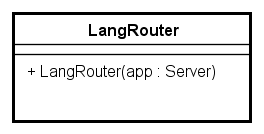
\includegraphics[scale=0.45]{UML/Classi/Back-End/QuizziPedia_Back-End_App_Routers_LangRouter.png}
	\caption{QuizziPedia::Back-End::App::Routers::LangRouter}
\end{figure}
\FloatBarrier
	\begin{itemize}
		\item \textbf{Descrizione} \\
		Classe che gestisce le richieste relative alla lingua.
		\item \textbf{Utilizzo} \\
		Viene utilizzata per chiamare il controller che si occupa di cambiare la lingua dell'applicazione.
		\item \textbf{Relazioni con altre classi}
			\begin{itemize}
				\item \textbf{IN \texttt{Server}} \\
				Classe che avvia il server. Nello specifico apre una connessione al database tramite \textit{Mongoose\ped{G}}, invoca il middleware\ped{G} \textit{Express\ped{G}} passando un riferimento al database MongoDB come parametro in modo che possa configurarsi con esso, invoca il middleware\ped{G} \textit{Passport\ped{G}} ed infine si mette in ascolto su una determinata porta. è il componente \textit{client\ped{G}} del pattern \textit{Chain of responsability\ped{G}}. Utilizza i moduli \textit{Mongoose\ped{G}}, \textit{Express\ped{G}}, \textit{Passport\ped{G}}.
				\item \textbf{OUT \texttt{NotFoundHandler}} \\
				Classe che si occupa della gestione dell'errore di una pagina non trovata. Componente ConcreteHandler del design pattern Chain of responsability.
			\end{itemize}
		\item \textbf{Metodi}
			\begin{itemize}
				\item \texttt{+ LangRouter(app: Server)} \\
				Contiene diverse ruote che vengono configurate all'avvio del server. Quest'ultime ricevono le richieste del \textit{client\ped{G}} e passano il controllo al ConcreteHandler successivo. \\
				\textbf{Parametri}:
					\begin{itemize}
						\item \texttt{app: Server} \\
						Rappresenta l'istanza del server su cui configurare i ruote che mappano i controllers specifici.
					\end{itemize}
			\end{itemize}
	\end{itemize}
